\documentclass[@CLASSOPTIONS@]{tumarticle}


\usepackage{cite}
\usepackage{multirow}
\usepackage{graphicx}
\usepackage{hyperref}
\usepackage{csquotes}


\title{Handwritten Mathematical Formula Detection using Convolutional Neural Networks}

\author[affil={1}, email={niklas.schweiger@tum.de}]{Niklas Schweiger}
\author[affil={1}, email={jannik.obenhoff@tum.de}]{Jannik Obenhoff}

\affil{Department of Electrical and Computer Engineering, Technical
  University of Munich, Arcisstr. 21, 80333 Munich, Germany}

\begin{document}
\twocolumn

\maketitle
\begin{abstract}
  In this analysis project, a data set~\cite{kaggledataset} containing numbers, mathematical
  symbols and letters has been processed in order to train a deep neural network (DNN) that
  serves as a mathematical formula classifier model.
  The final model is applied to real handwritten formulas over a plotly dashboard to demonstrate the model
  performance in the real-world use case.

\end{abstract}

\section{Introduction}

Handwritten formula detection is a challenging problem in the field of pattern recognition and
image processing.
Despite the recent advancements in machine learning algorithms, different styles, sizes and character
shapes make it difficult to find a perfect detection model.
In this paper, we present an approach to handwritten formula detection using convolutional
neural networks (CNNs), image processing, and feature extraction to achieve the best possible results
in real world scenarios.

\section{Data}
\label{sec:measures}

This section describes the essential preprocessing that has had to be done to the raw
data set~\cite{kaggledataset} before handing it over to the CNN,
as well as the image processing methods for the real world data.

\subsection{Training Data}
\subsubsection{Understanding and Cleaning the Data}

The initial training dataset contains over 370,000 image samples, each in the 45x45 jpeg file format.
The first step was to reduce the dataset to the characters essential for the
implemented mathematical functionalities (see~\ref{subsec:dash}),
thus yielding a data set of 300,000 image samples.

\subsubsection{Preprocessing the Data}

The optimal image size to train the CNN would be 28x28 pixels, a good compromise between
memory complexity and detail loss.
In this case a higher resolution is not needed, as the subject of the images are rather simple.

After scaling down the samples and first tests, the results were not as desired.
The next preprocessing step was to widen the line thickness of each character.
After some back and forth the optimal line thickness was 6 pixels for the 45x45 jpg samples and
4 pixels for the down sampled 28x28 images as well as adding a white border of 20\% on each side.
Compare Figure~\ref{Fig:Data1} and Figure~\ref{Fig:Data2}.

\begin{figure}[!htb]
   \begin{minipage}{0.24\textwidth}
     \centering
     \fbox{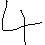
\includegraphics[width=.7\linewidth]{figures/4_clean}}
     \caption{Raw Data}\label{Fig:Data1}
   \end{minipage}\hfill
   \begin{minipage}{0.24\textwidth}
     \centering
     \fbox{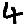
\includegraphics[width=.7\linewidth]{figures/4_sampled}}
     \caption{Processed Data}\label{Fig:Data2}
   \end{minipage}
\end{figure}

\subsection{Real Data}
\label{subsec:realdata}
Before handing the real-world data to the CNN the submitted image needs
to be transformed in order to achieve the best possible results.
The raw input data is a photo of a handwritten mathematical formula, preferable on white paper
and written in dark color.

\subsubsection{Adaptive Thresholding}

To eliminate distracting background noise and to separate the desired foreground formula
from the background based on the difference in pixel intensities of each region,
an adaptive threshold is applied to the image~\cite{threshold}.
For each pixel in the submitted image, a threshold has to be calculated with the following operations.
The first steps are two convolutions with a gaussian kernel with side length of seven (Figure ~\ref{Fig:Data4_1}).
Following the convolution, each value of the image array gets subtracted by 50 minus the minimum
pixel value (Min) of the original image.
The last step is to threshold the original image with the obtained threshold image.
The outcome of this process is an image only containing black and white pixels, as illustrated in Figure~\ref{Fig:Data4}.

\begin{figure}[!htb]
    \vspace{0.3cm}
   \begin{minipage}{0.48\textwidth}
     \centering
     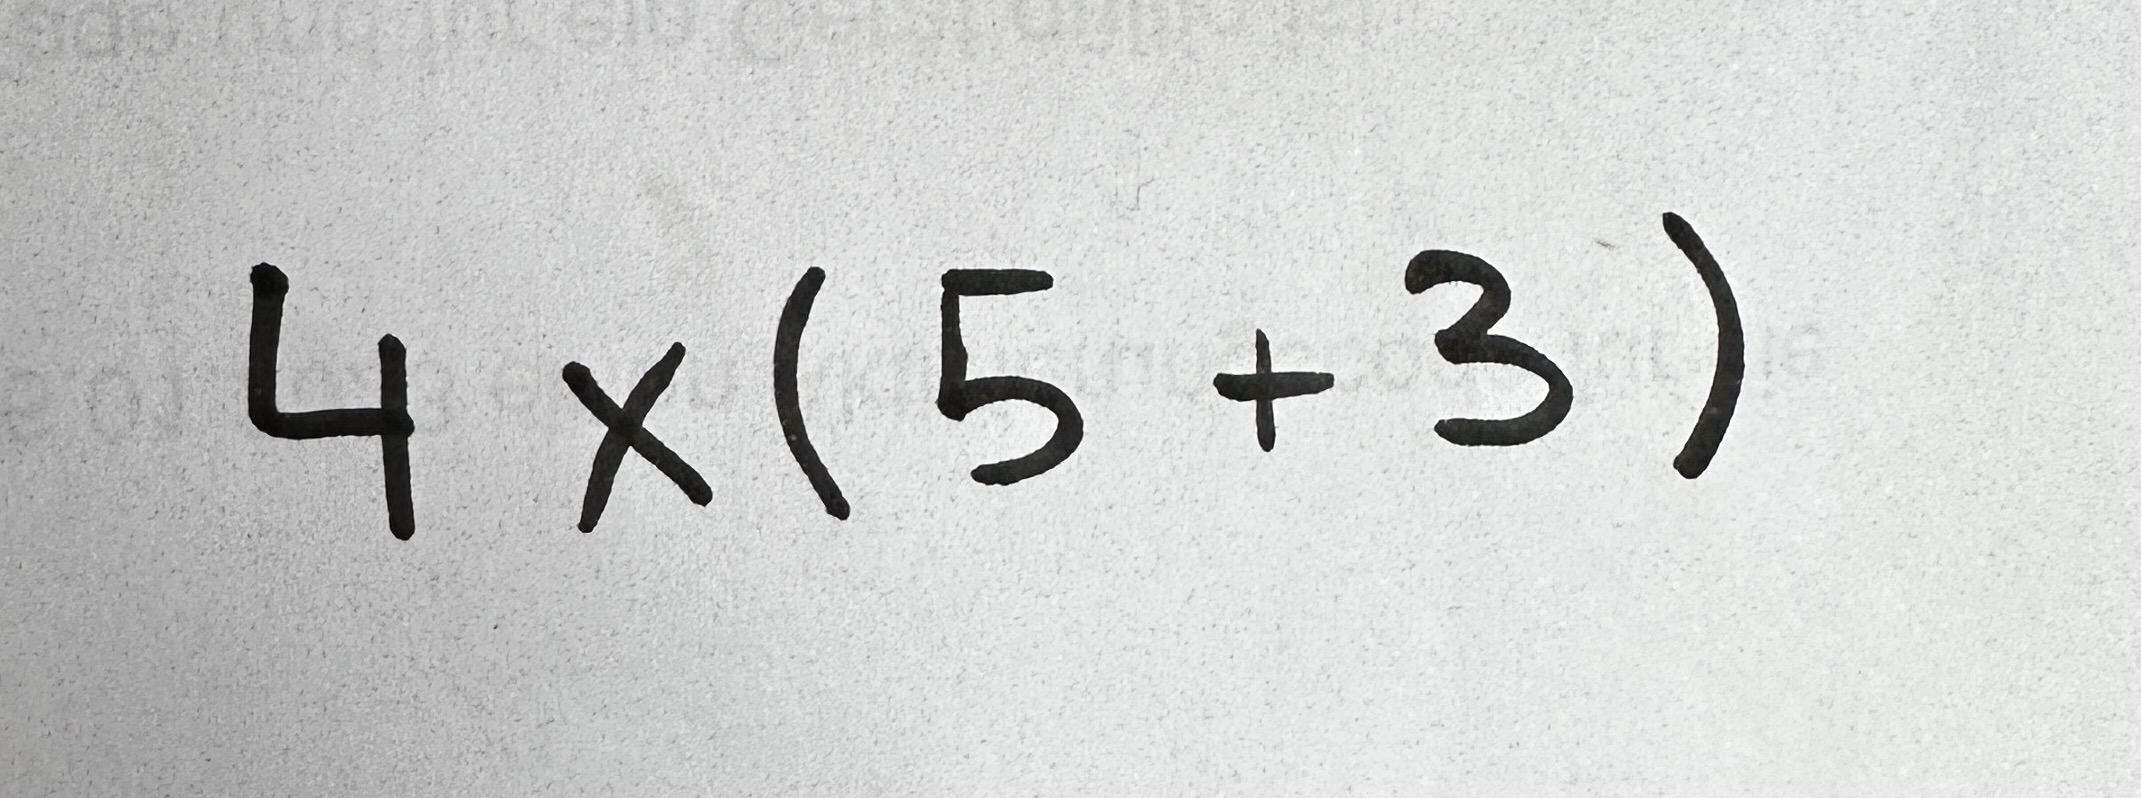
\includegraphics[width=.7\linewidth]{figures/real_data_1}
     \caption{Input Image}\label{Fig:Data3}
   \end{minipage}\hfill
   \vspace{0.3cm}
   \begin{minipage}{0.48\textwidth}
     \centering
     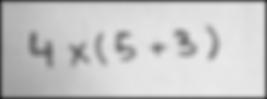
\includegraphics[width=.7\linewidth]{figures/convolve}
     \caption{After Convolution}\label{Fig:Data4_1}
   \end{minipage}
      \vspace{0.3cm}

   \begin{minipage}{0.48\textwidth}
     \centering
     \fbox{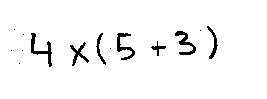
\includegraphics[width=.67\linewidth]{figures/real_data_2}}
     \caption{After Thresholding}\label{Fig:Data4}
   \end{minipage}
  \hfill
   \begin{minipage}{0.48\textwidth}
     \centering
     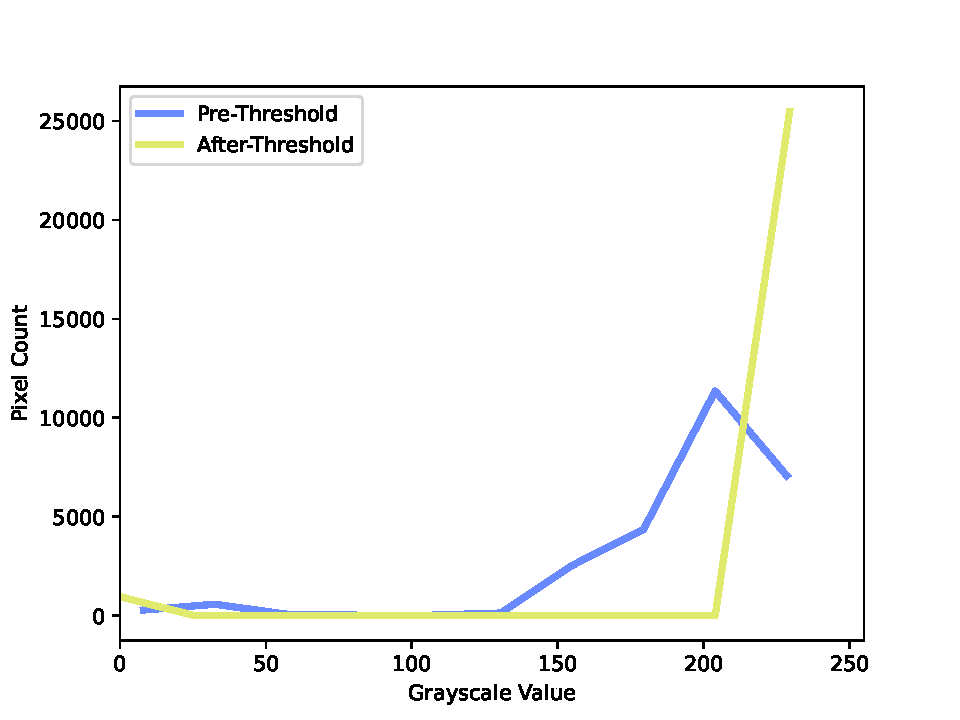
\includegraphics[width=.9\linewidth]{figures/histogram}
     \caption{Pixel Distribution Histogram}\label{Fig:Data5}
   \end{minipage}
\end{figure}

\subsubsection{Scanning and Sampling}

The next step is to scan the image obtaining all individual characters.
The image array, only containing black and white values, gets scanned by columns first to find the starting
and ending column of each character.
To eliminate possible noise, characters only containing one or two columns are being deleted.
After column search, height search is applied to find the character baseline and height.
Every character column gets reduced in size to the maximal height and minimal baseline found in height search.
The second last step is to remove potential characters with a threshold dimension shape of\\
min(shape)/max(shape) < 0.1.
The final step is to add an artificial border and to resize every character to a 28x28 image to
perfectly fit the training dataset.
The final result can be seen in Figure~\ref{Fig:Data6}.

\begin{figure}
    \begin{minipage}{0.48\textwidth}
     \centering
     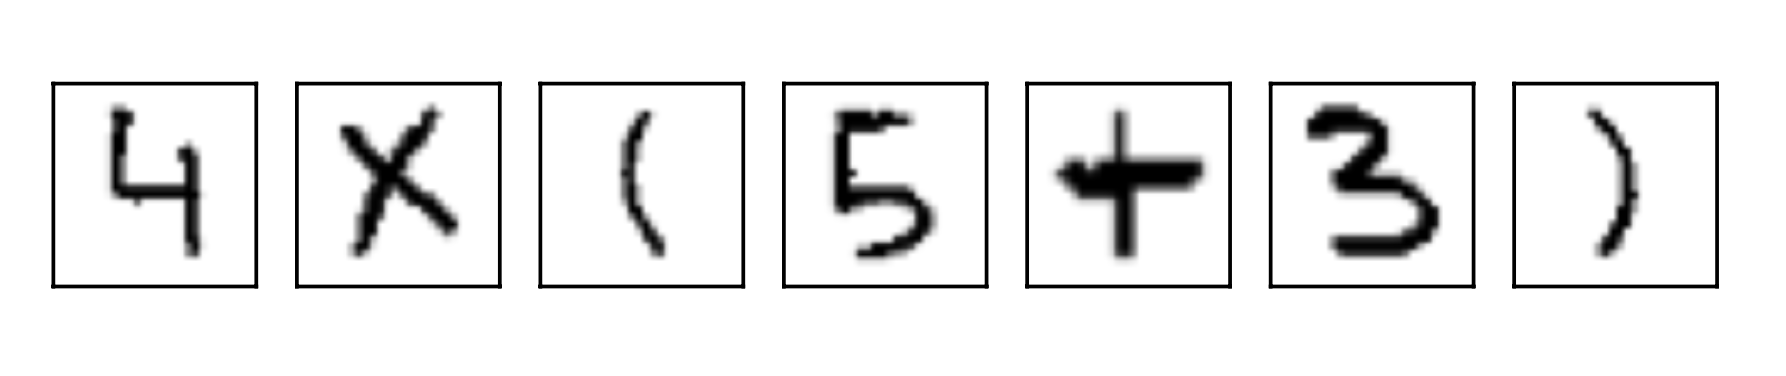
\includegraphics[width=.9\linewidth]{figures/real_data_3}
     \caption{Individual Characters after Scanning}\label{Fig:Data6}
   \end{minipage}
\end{figure}

\section{Model}
\label{sec:implementation}


\subsection{Theoretical background}

For this classification problem a Convolutional Neural Network is being employed.
As a specific type of Deep Neural Network, a CNN fits under the definition of a supervised learning model as the correct
labels are always available for the Network.
The main advantages of CNNs are their use of local connectivity and shared weights.
CNNs use convolutional layers that are specifically designed to take advantage of the spatial relationship between
adjacent pixels in an image.
By using local connectivity, CNNs are able to learn features that are translation invariant, meaning they can
recognize the same feature in different parts of an image.
The shared weights approach reduces the number of parameters in the model by using the same weights for each part of the
image, which makes the training process faster and more efficient~\cite{reviewDL}.
Also, CNNs often use pooling layers like Max or Average Pooling in order to reduce the dimensionality of the feature maps,
which further reduces the computational cost and helps to avoid overfitting.
For these reasons CNNs are very suitable for image recognition but also find applications in speech
processing.
In fact, well-trained CNNs have been shown to outperform humans on certain image classification tasks.

\begin{figure}
    \begin{minipage}{0.48\textwidth}
     \centering
     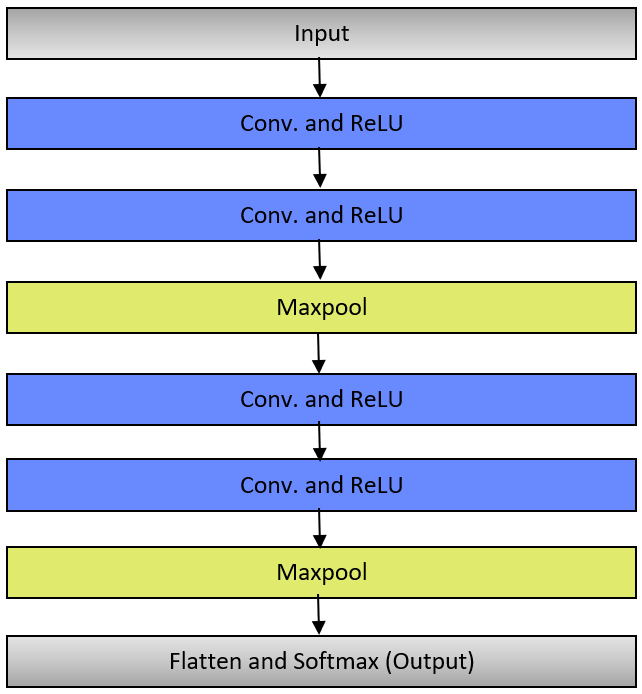
\includegraphics[width=.9\linewidth]{figures/CNN_Arch_5}
     \caption{Architecture of the CNN}\label{Fig:CNN_A}
   \end{minipage}
\end{figure}

\subsection{Architecture}

The model that has been used for this project is a CNN with a total of six layers, which structure is depicted in
figure~\ref{Fig:CNN_A}.
Given that only monochromatic images are fed into the network, the input size, specifically the number of channels,
was specified as one, as opposed to the three channels that would typically be utilized for RGB images.
Each of the following hidden layers consists of thirty-two neurons.
In the first layer each neuron convolves the input tensor (28x28x1) with a kernel of size three, a stride of one, and
a padding of one.
The Rectified Linear Unit (ReLU) function is applied as activation after the convolution.
The second layer follows a similar structure, where convolution and ReLU activation are performed, followed by a MaxPool
layer with stride and padding of two, resulting in a (14x14x1) tensor at each neuron.
The same three-layer structure is then applied for layers four, five and six which results in thirty-two (7x7x1) tensors for
layer six.
As the Softmax function requires one-dimensional input, the three-dimensional tensors are flattened into a (1568) array.
Finally, the SoftMax function evaluates a probability for each output class.

\begin{figure}
    \begin{minipage}{0.48\textwidth}
     \centering
     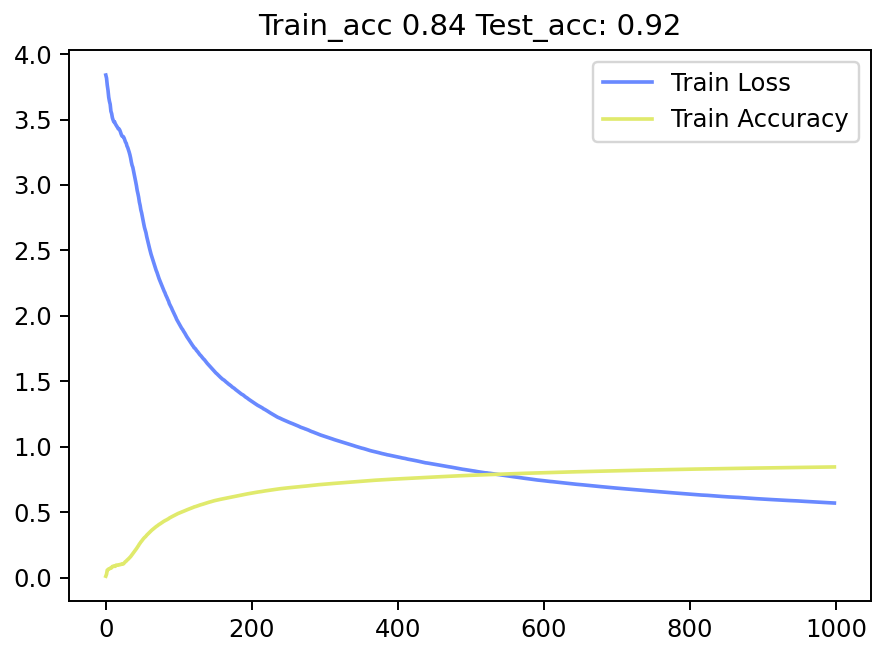
\includegraphics[width=.9\linewidth]{figures/train_plot}
     \caption{Train Loss and Train Accuracy}\label{Fig:tp}
   \end{minipage}
\end{figure}

\subsection{Training}

In order to train the network Cross Entropy Loss was utilized as it demonstrates exceptional efficacy with probabilistic
methods in the neural network SoftMax as well as in classification problems in overall.
Due to its low computational cost and fast convergence the adaptive moment estimation Adam~\cite{Adam} was used as the optimization
function with a learning rate of 0.001.\\
Despite its small size with only a few layers and no data augmentation, the Network performs well on the given dataset,
achieving a Training accuracy of 0.86 and Test accuracy of 0.92 after training only on a thousand images, as shown in
figure ~\ref{Fig:tp}.\\
Upon completion of three training epochs utilizing a comprehensive dataset consisting of over 200,000 images, in
addition to a test dataset consisting of over 100,000 images, the network achieved a remarkable test accuracy of 96 percent.
This outcome is deemed highly satisfactory for the given project, as even for the authors, the identification of certain
images presented a challenge.\\

\subsubsection{Data Augmentation}
Data augmentation often has the ability to significantly improve the performance of a network but in this case, it
was not useful, as the dataset is already very large with over 300,000 images with a specific format and coloring for
the detected images.
As an illustration, implementing conventional data augmentation techniques, such as image rotation or brightness
modification~\cite{DataAugm}, would not be of significant benefit.
This is due to the inherent characteristics of the symbols, which are generally already correctly oriented and
preprocessed in such a way that the pixels only contain two grayscale values for black and white.
While standard data augmentation techniques were evaluated in the project, they were found to be ineffective in
improving network performance and, in fact, were observed to have a detrimental effect.

\section{Performance and Results}
\label{sec:customization}

\subsection{Dashboard}
\label{subsec:dash}
To make easy handling possible a Plotly~\cite{plotly} Dashboard is being used (Figure~\ref{Fig:Dash}).
The dashboard design is kept minimal to maximize the user experience.
The first step for a user is to select a functionality.
\begin{itemize}
\item Basic calculations using numbers and simple mathematical operations.
\item Plotting a function containing one variable\\ (Figure~\ref{Fig:Dash2}).
\item Solving mathematical equations containing variables by accessing the
Wolfram Alpha Api~\cite{wolfram}.
\end{itemize}
Afterwards you can upload a photo of the handwritten formula or even take a photo
with the webcam.
The submitted image gets processed accordingly to the techniques from section (2.2\nameref{subsec:realdata}),
the individual detected characters get displayed, and the user can make a reselection
in the case that noise or other undesired parts have been detected.
The final selection gets hand over to the model to classify the characters.
Depending on the selected functionality the result is being displayed.

\begin{figure}
    \begin{minipage}{0.48\textwidth}
     \centering
     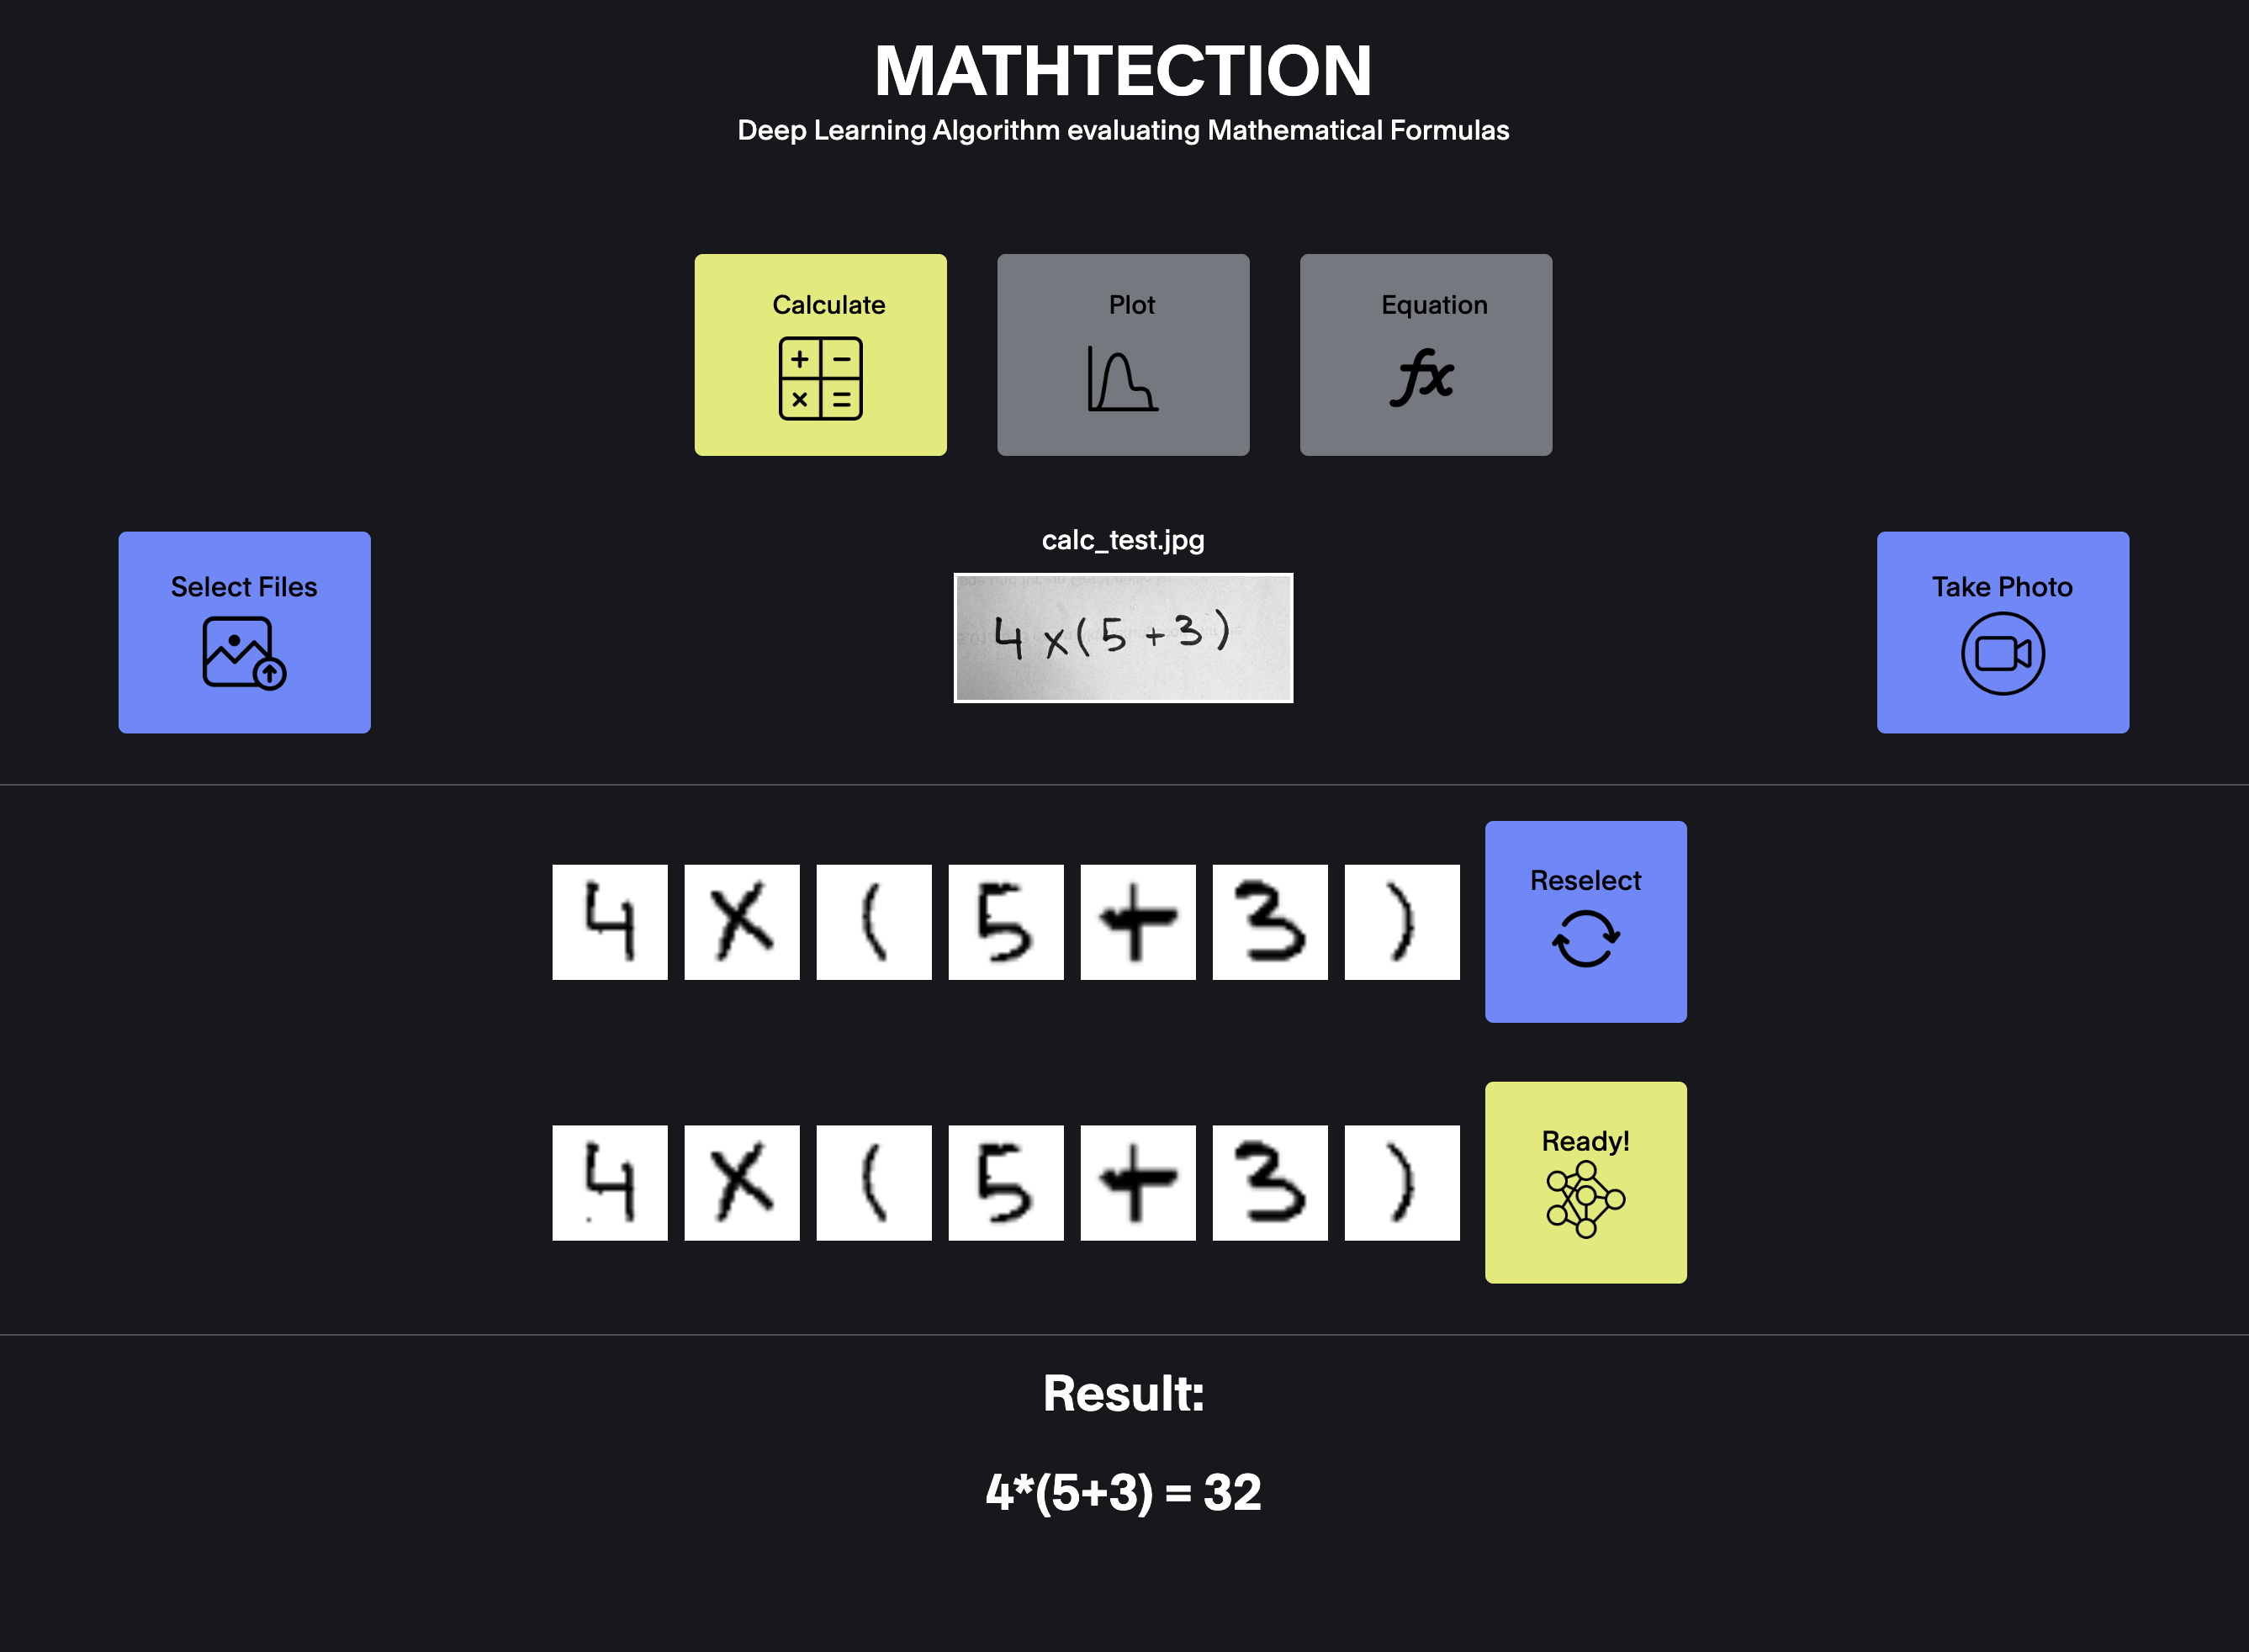
\includegraphics[width=.9\linewidth]{figures/dash}
     \caption{Plotly Dash}\label{Fig:Dash}
   \end{minipage}
\end{figure}
\begin{figure}
    \begin{minipage}{0.48\textwidth}
     \centering
     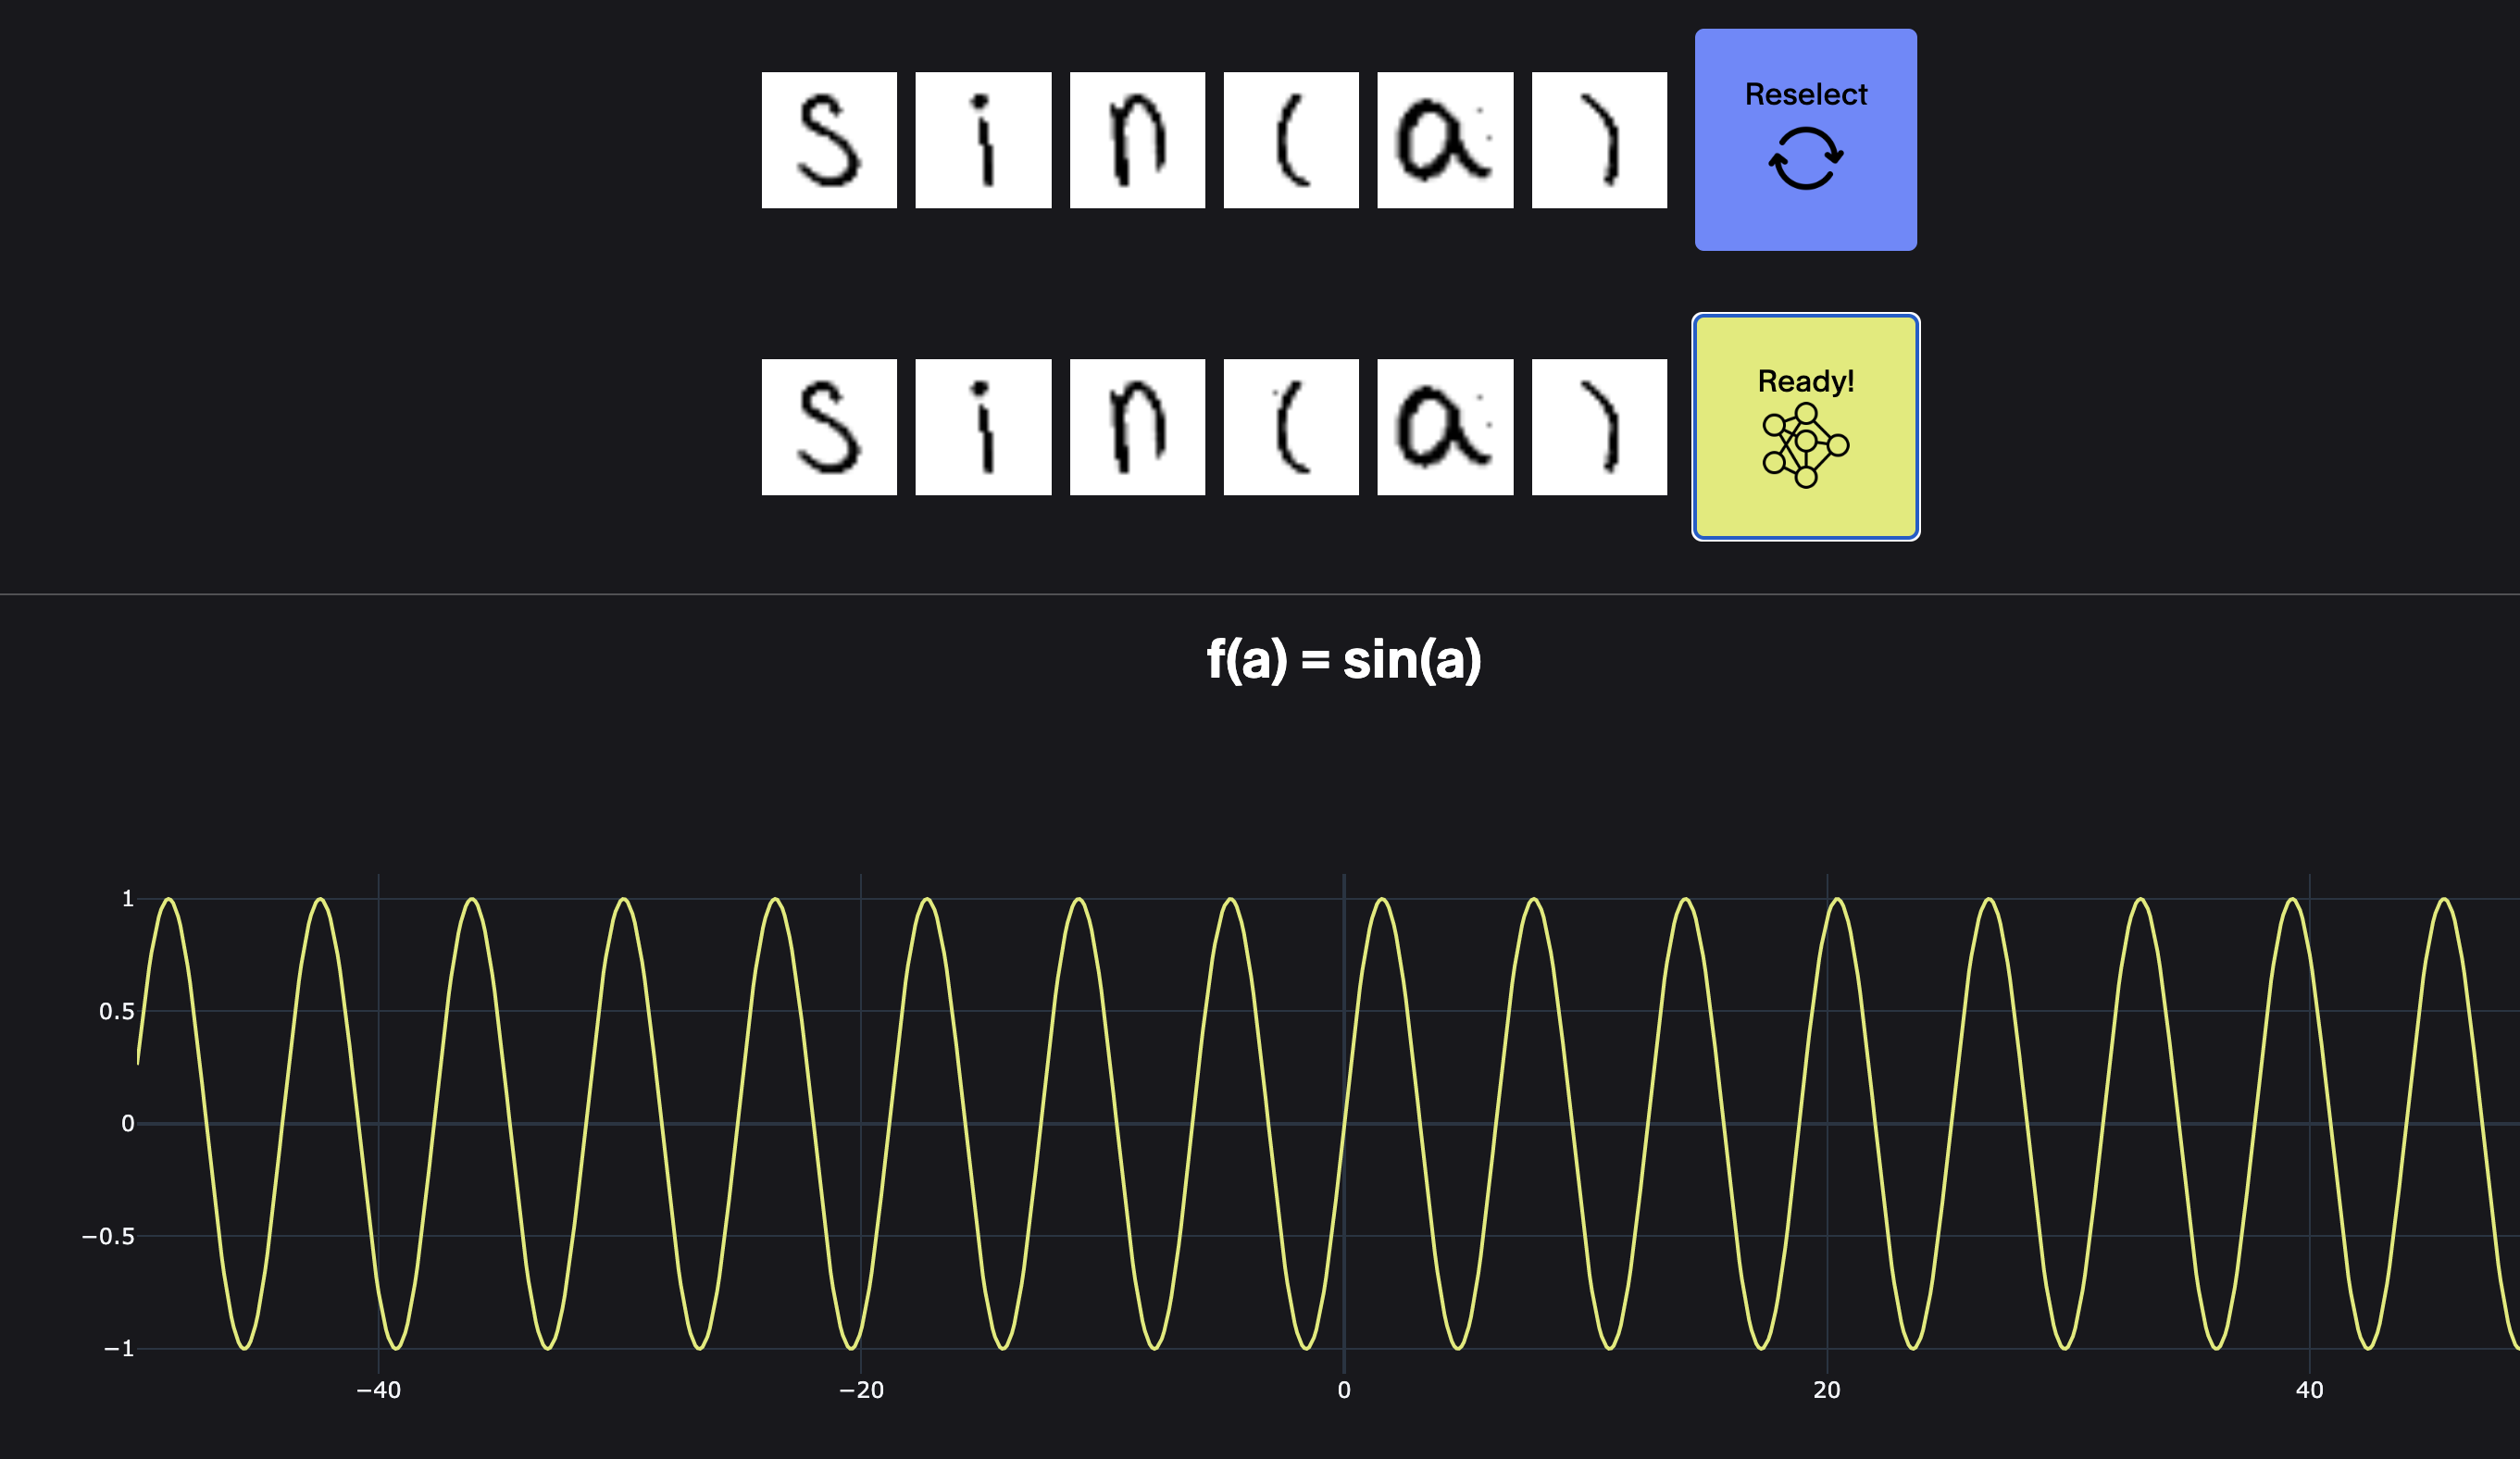
\includegraphics[width=.9\linewidth]{figures/dash3}
     \caption{Plot Functionality}\label{Fig:Dash2}
   \end{minipage}
\end{figure}

\subsection{Overall}

\section{Outlook and Improvements}

As the Network already has a good test accuracy on the given test set further improvements with a more complex Network
or by increasing the size of the hidden layers might increase the performance of the Network on the test set but would
not significantly change the performance of the Network when classifying real handwritten symbols.
Instead, training on a real human generated dataset of handwritten symbols would be a better option.

One approach to achieve this would be to collect the submitted formula images and utilize them to train the CNN\@.
Additionally, it may be beneficial to enhance the threshold and scanning process
to minimize the amount of inaccurately detected characters.

In the future, additional features could be added to the application,
such as support for more complex mathematical expressions, including integrals and fractions.
However, this would require a better image recognition and an improved CNN as a foundation.

\begin{thebibliography}{10}
  \newcommand{\enquote}[1]{``#1''}

  \bibitem{kaggledataset}
  Xai Nano, \emph{Kaggle Data set: Handwritten math symbols dataset}
  \url{https://www.kaggle.com/datasets/xainano/handwrittenmathsymbols}
  (last accessed: 20.02.2023).

  \bibitem{plotly}
  Plotly \url{https://plotly.com/dash/}
  (last accessed: 07.03.2023).

  \bibitem{threshold}
  R. Fisher, S. Perkins, A. Walker, E. Wolfart.
  \emph{Adaptive Thresholding}
  \url{https://homepages.inf.ed.ac.uk/rbf/HIPR2/adpthrsh.htm}
  (last accessed: 08.03.2023).

  \bibitem{hunt1999pragmatic}
  A.~Hunt and H.~Thomas, \emph{The Pragmatic Programmer: From Journeyman to
    Master} (Addison-Wesley, Boston, 1999), 1st ed.

  \bibitem{prlic2012}
  A.~Prli{\'c} and J.~B. Procter, \enquote{Ten simple rules for the open
    development of scientific software,} PLoS Comput. Biol. \textbf{8}, 1--3
  (2012).

  \bibitem{reviewDL}
  L.Alzubaidi, J. Zhang, A. Humaidi, A. Al-Dajuaili, Y. Duan, O. Al-Shamma, J. Santamaria, M.Fadhel, M. Al-Amidie, L. Farhan,
    \emph{Review of deep learning: concepts, CNN architectures, challenges, applications, future directions}
    \url{https://journalofbigdata.springeropen.com/articles/10.1186/s40537-021-00444-8}
    (last accessed 07.03.2023).

  \bibitem{Adam}
  D. Kingma, J.Lei Ba, \emph{ADAM: A method for stochastic optimization page 6--7}
    \url{https://arxiv.org/pdf/1412.6980.pdf}
        (last accessed 07.03.2023).

  \bibitem{DataAugm}
  J. Wang and L. Perez: \emph{The Effectiveness of Data Augmentation in Image Classification using Deep Learning}
    \url{https://arxiv.org/pdf/1712.04621.pdf}
    (kast accessed 07.03.2023)

  \bibitem{wolfram}
  Wolfram Alpha \url{https://www.wolframalpha.com/}
  (last accessed: 08.03.2023).



\end{thebibliography}

\end{document}
